\documentclass{standalone}
\usepackage{tikz}
\usetikzlibrary{patterns, positioning}

\begin{document}
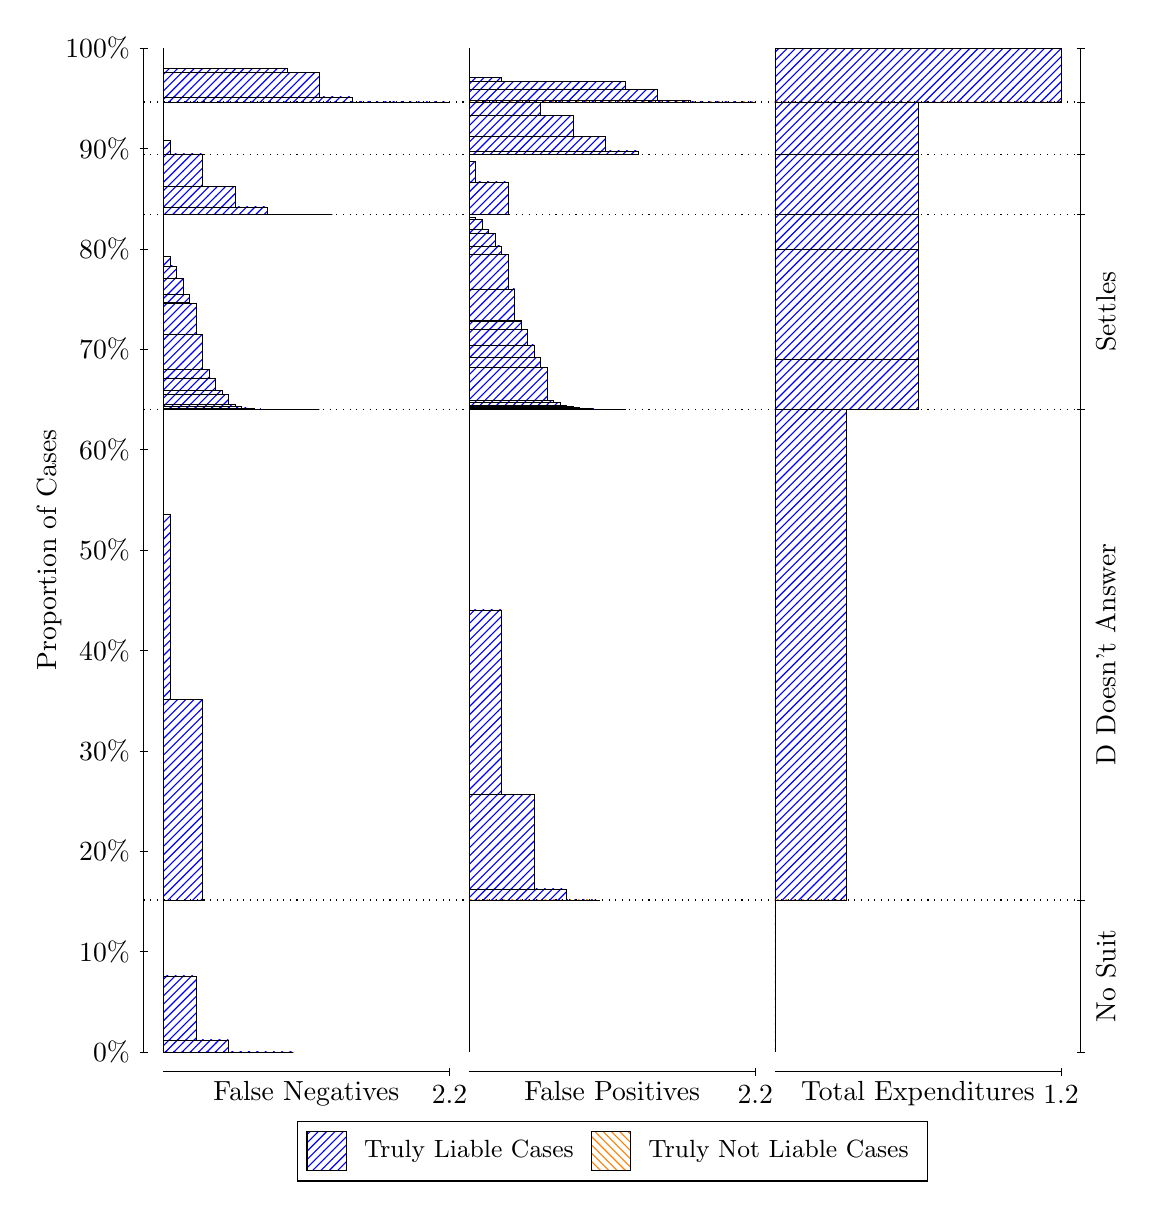
\begin{tikzpicture}
\draw[black, very thin] (1.5,1.75) -- (1.5,14.5);
\node[rotate=90, anchor=center] at (0.3, 8.125) {Proportion of Cases};
\draw[black, very thin] (1.45,1.75) -- (1.55,1.75);
\node[anchor=east] at (1.45, 1.75) {0\%};
\draw[black, very thin] (1.45,3.025) -- (1.55,3.025);
\node[anchor=east] at (1.45, 3.025) {10\%};
\draw[black, very thin] (1.45,4.3) -- (1.55,4.3);
\node[anchor=east] at (1.45, 4.3) {20\%};
\draw[black, very thin] (1.45,5.575) -- (1.55,5.575);
\node[anchor=east] at (1.45, 5.575) {30\%};
\draw[black, very thin] (1.45,6.85) -- (1.55,6.85);
\node[anchor=east] at (1.45, 6.85) {40\%};
\draw[black, very thin] (1.45,8.125) -- (1.55,8.125);
\node[anchor=east] at (1.45, 8.125) {50\%};
\draw[black, very thin] (1.45,9.4) -- (1.55,9.4);
\node[anchor=east] at (1.45, 9.4) {60\%};
\draw[black, very thin] (1.45,10.675) -- (1.55,10.675);
\node[anchor=east] at (1.45, 10.675) {70\%};
\draw[black, very thin] (1.45,11.95) -- (1.55,11.95);
\node[anchor=east] at (1.45, 11.95) {80\%};
\draw[black, very thin] (1.45,13.225) -- (1.55,13.225);
\node[anchor=east] at (1.45, 13.225) {90\%};
\draw[black, very thin] (1.45,14.5) -- (1.55,14.5);
\node[anchor=east] at (1.45, 14.5) {100\%};

\draw[black, very thin] (13.4,1.75) -- (13.4,14.5);
\draw[black, very thin] (13.35,1.75) -- (13.45,1.75);
\node[anchor=west] at (13.35, 1.75) {};
\draw[black, very thin] (13.35,3.6805) -- (13.45,3.6805);
\node[anchor=west] at (13.35, 3.6805) {};
\draw[black, very thin] (13.35,9.913) -- (13.45,9.913);
\node[anchor=west] at (13.35, 9.913) {};
\draw[black, very thin] (13.35,12.386) -- (13.45,12.386);
\node[anchor=west] at (13.35, 12.386) {};
\draw[black, very thin] (13.35,13.153) -- (13.45,13.153);
\node[anchor=west] at (13.35, 13.153) {};
\draw[black, very thin] (13.35,13.815) -- (13.45,13.815);
\node[anchor=west] at (13.35, 13.815) {};
\draw[black, very thin] (13.35,14.5) -- (13.45,14.5);
\node[anchor=west] at (13.35, 14.5) {};

\draw[black, very thin, pattern color=blue, pattern=north east lines] (1.75,1.75) rectangle (3.4015,1.75);
\draw[black, very thin, pattern color=blue, pattern=north east lines] (1.75,1.75) rectangle (2.9886,1.7513);
\draw[black, very thin, pattern color=blue, pattern=north east lines] (1.75,1.7513) rectangle (2.5758,1.9045);
\draw[black, very thin, pattern color=blue, pattern=north east lines] (1.75,1.9045) rectangle (2.1629,2.7166);
\draw[black, very thin, pattern color=orange, pattern=north west lines] (1.75,2.7166) rectangle (1.75,2.7166);
\draw[black, very thin, pattern color=blue, pattern=north east lines] (1.75,2.7166) rectangle (1.75,3.6805);
\draw[black, very thin, pattern color=blue, pattern=north east lines] (1.75,3.6805) rectangle (2.2455,6.2283);
\draw[black, very thin, pattern color=blue, pattern=north east lines] (1.75,6.2283) rectangle (1.8326,8.5731);
\draw[black, very thin, pattern color=orange, pattern=north west lines] (1.75,8.5731) rectangle (1.75,8.5731);
\draw[black, very thin, pattern color=blue, pattern=north east lines] (1.75,8.5731) rectangle (1.75,9.913);
\draw[black, very thin, pattern color=blue, pattern=north east lines] (1.75,9.913) rectangle (3.7318,9.913);
\draw[black, very thin, pattern color=blue, pattern=north east lines] (1.75,9.913) rectangle (3.5667,9.913);
\draw[black, very thin, pattern color=blue, pattern=north east lines] (1.75,9.913) rectangle (3.4015,9.913);
\draw[black, very thin, pattern color=blue, pattern=north east lines] (1.75,9.913) rectangle (3.3189,9.913);
\draw[black, very thin, pattern color=blue, pattern=north east lines] (1.75,9.913) rectangle (3.2364,9.913);
\draw[black, very thin, pattern color=blue, pattern=north east lines] (1.75,9.913) rectangle (3.2364,9.913);
\draw[black, very thin, pattern color=blue, pattern=north east lines] (1.75,9.913) rectangle (3.1538,9.9131);
\draw[black, very thin, pattern color=blue, pattern=north east lines] (1.75,9.9131) rectangle (3.0712,9.9131);
\draw[black, very thin, pattern color=blue, pattern=north east lines] (1.75,9.9131) rectangle (2.9886,9.9173);
\draw[black, very thin, pattern color=blue, pattern=north east lines] (1.75,9.9173) rectangle (2.9061,9.925);
\draw[black, very thin, pattern color=blue, pattern=north east lines] (1.75,9.925) rectangle (2.8235,9.925);
\draw[black, very thin, pattern color=blue, pattern=north east lines] (1.75,9.925) rectangle (2.8235,9.9302);
\draw[black, very thin, pattern color=blue, pattern=north east lines] (1.75,9.9302) rectangle (2.7409,9.9302);
\draw[black, very thin, pattern color=blue, pattern=north east lines] (1.75,9.9302) rectangle (2.7409,9.9507);
\draw[black, very thin, pattern color=blue, pattern=north east lines] (1.75,9.9507) rectangle (2.6583,9.9715);
\draw[black, very thin, pattern color=blue, pattern=north east lines] (1.75,9.9715) rectangle (2.5758,10.103);
\draw[black, very thin, pattern color=blue, pattern=north east lines] (1.75,10.103) rectangle (2.4932,10.103);
\draw[black, very thin, pattern color=blue, pattern=north east lines] (1.75,10.103) rectangle (2.4932,10.15);
\draw[black, very thin, pattern color=blue, pattern=north east lines] (1.75,10.15) rectangle (2.4106,10.151);
\draw[black, very thin, pattern color=blue, pattern=north east lines] (1.75,10.151) rectangle (2.4106,10.312);
\draw[black, very thin, pattern color=blue, pattern=north east lines] (1.75,10.312) rectangle (2.4106,10.312);
\draw[black, very thin, pattern color=blue, pattern=north east lines] (1.75,10.312) rectangle (2.328,10.312);
\draw[black, very thin, pattern color=blue, pattern=north east lines] (1.75,10.312) rectangle (2.328,10.415);
\draw[black, very thin, pattern color=blue, pattern=north east lines] (1.75,10.415) rectangle (2.2455,10.86);
\draw[black, very thin, pattern color=blue, pattern=north east lines] (1.75,10.86) rectangle (2.1629,11.259);
\draw[black, very thin, pattern color=blue, pattern=north east lines] (1.75,11.259) rectangle (2.0803,11.267);
\draw[black, very thin, pattern color=blue, pattern=north east lines] (1.75,11.267) rectangle (2.0803,11.372);
\draw[black, very thin, pattern color=blue, pattern=north east lines] (1.75,11.372) rectangle (1.9977,11.377);
\draw[black, very thin, pattern color=blue, pattern=north east lines] (1.75,11.377) rectangle (1.9977,11.57);
\draw[black, very thin, pattern color=blue, pattern=north east lines] (1.75,11.57) rectangle (1.9977,11.57);
\draw[black, very thin, pattern color=blue, pattern=north east lines] (1.75,11.57) rectangle (1.9152,11.578);
\draw[black, very thin, pattern color=blue, pattern=north east lines] (1.75,11.578) rectangle (1.9152,11.732);
\draw[black, very thin, pattern color=blue, pattern=north east lines] (1.75,11.732) rectangle (1.8326,11.854);
\draw[black, very thin, pattern color=orange, pattern=north west lines] (1.75,11.854) rectangle (1.75,11.854);
\draw[black, very thin, pattern color=blue, pattern=north east lines] (1.75,11.854) rectangle (1.75,12.386);
\draw[black, very thin, pattern color=blue, pattern=north east lines] (1.75,12.386) rectangle (3.897,12.386);
\draw[black, very thin, pattern color=blue, pattern=north east lines] (1.75,12.386) rectangle (3.4841,12.386);
\draw[black, very thin, pattern color=blue, pattern=north east lines] (1.75,12.386) rectangle (3.0712,12.483);
\draw[black, very thin, pattern color=blue, pattern=north east lines] (1.75,12.483) rectangle (2.6583,12.739);
\draw[black, very thin, pattern color=blue, pattern=north east lines] (1.75,12.739) rectangle (2.2455,13.153);
\draw[black, very thin, pattern color=orange, pattern=north west lines] (1.75,13.153) rectangle (1.75,13.153);
\draw[black, very thin, pattern color=blue, pattern=north east lines] (1.75,13.153) rectangle (2.2455,13.155);
\draw[black, very thin, pattern color=blue, pattern=north east lines] (1.75,13.155) rectangle (1.8326,13.327);
\draw[black, very thin, pattern color=orange, pattern=north west lines] (1.75,13.327) rectangle (1.75,13.327);
\draw[black, very thin, pattern color=blue, pattern=north east lines] (1.75,13.327) rectangle (1.75,13.815);
\draw[black, very thin, pattern color=blue, pattern=north east lines] (1.75,13.815) rectangle (5.3833,13.815);
\draw[black, very thin, pattern color=blue, pattern=north east lines] (1.75,13.815) rectangle (4.9705,13.815);
\draw[black, very thin, pattern color=blue, pattern=north east lines] (1.75,13.815) rectangle (4.5576,13.817);
\draw[black, very thin, pattern color=blue, pattern=north east lines] (1.75,13.817) rectangle (4.1447,13.88);
\draw[black, very thin, pattern color=blue, pattern=north east lines] (1.75,13.88) rectangle (3.7318,14.188);
\draw[black, very thin, pattern color=blue, pattern=north east lines] (1.75,14.188) rectangle (3.3189,14.239);
\draw[black, very thin, pattern color=blue, pattern=north east lines] (1.75,14.239) rectangle (2.9886,14.239);
\draw[black, very thin, pattern color=blue, pattern=north east lines] (1.75,14.239) rectangle (2.9061,14.239);
\draw[black, very thin, pattern color=blue, pattern=north east lines] (1.75,14.239) rectangle (2.5758,14.239);
\draw[black, very thin, pattern color=blue, pattern=north east lines] (1.75,14.239) rectangle (2.1629,14.244);
\draw[black, very thin, pattern color=orange, pattern=north west lines] (1.75,14.244) rectangle (1.75,14.244);
\draw[black, very thin, pattern color=blue, pattern=north east lines] (1.75,14.244) rectangle (1.75,14.5);
\draw[black, very thin, pattern color=orange, pattern=north west lines] (5.6333,1.75) rectangle (5.6333,1.75);
\draw[black, very thin, pattern color=blue, pattern=north east lines] (5.6333,1.75) rectangle (5.6333,3.6805);
\draw[black, very thin, pattern color=orange, pattern=north west lines] (5.6333,3.6805) rectangle (7.2848,3.6805);
\draw[black, very thin, pattern color=blue, pattern=north east lines] (5.6333,3.6805) rectangle (7.2848,3.6817);
\draw[black, very thin, pattern color=blue, pattern=north east lines] (5.6333,3.6817) rectangle (6.872,3.8211);
\draw[black, very thin, pattern color=blue, pattern=north east lines] (5.6333,3.8211) rectangle (6.4591,5.0204);
\draw[black, very thin, pattern color=blue, pattern=north east lines] (5.6333,5.0204) rectangle (6.0462,7.3652);
\draw[black, very thin, pattern color=blue, pattern=north east lines] (5.6333,7.3652) rectangle (5.6333,9.913);
\draw[black, very thin, pattern color=orange, pattern=north west lines] (5.6333,9.913) rectangle (7.6152,9.913);
\draw[black, very thin, pattern color=blue, pattern=north east lines] (5.6333,9.913) rectangle (7.6152,9.9143);
\draw[black, very thin, pattern color=orange, pattern=north west lines] (5.6333,9.9143) rectangle (7.45,9.9143);
\draw[black, very thin, pattern color=blue, pattern=north east lines] (5.6333,9.9143) rectangle (7.45,9.9156);
\draw[black, very thin, pattern color=orange, pattern=north west lines] (5.6333,9.9156) rectangle (7.2848,9.9156);
\draw[black, very thin, pattern color=blue, pattern=north east lines] (5.6333,9.9156) rectangle (7.2848,9.9181);
\draw[black, very thin, pattern color=blue, pattern=north east lines] (5.6333,9.9181) rectangle (7.2023,9.9217);
\draw[black, very thin, pattern color=orange, pattern=north west lines] (5.6333,9.9217) rectangle (7.1197,9.9217);
\draw[black, very thin, pattern color=blue, pattern=north east lines] (5.6333,9.9217) rectangle (7.1197,9.9277);
\draw[black, very thin, pattern color=blue, pattern=north east lines] (5.6333,9.9277) rectangle (7.0371,9.9315);
\draw[black, very thin, pattern color=orange, pattern=north west lines] (5.6333,9.9315) rectangle (6.9545,9.9315);
\draw[black, very thin, pattern color=blue, pattern=north east lines] (5.6333,9.9315) rectangle (6.9545,9.9468);
\draw[black, very thin, pattern color=blue, pattern=north east lines] (5.6333,9.9468) rectangle (6.872,9.96);
\draw[black, very thin, pattern color=orange, pattern=north west lines] (5.6333,9.96) rectangle (6.7894,9.96);
\draw[black, very thin, pattern color=blue, pattern=north east lines] (5.6333,9.96) rectangle (6.7894,9.9975);
\draw[black, very thin, pattern color=blue, pattern=north east lines] (5.6333,9.9975) rectangle (6.7068,10.025);
\draw[black, very thin, pattern color=blue, pattern=north east lines] (5.6333,10.025) rectangle (6.6242,10.026);
\draw[black, very thin, pattern color=orange, pattern=north west lines] (5.6333,10.026) rectangle (6.6242,10.026);
\draw[black, very thin, pattern color=blue, pattern=north east lines] (5.6333,10.026) rectangle (6.6242,10.445);
\draw[black, very thin, pattern color=blue, pattern=north east lines] (5.6333,10.445) rectangle (6.5417,10.567);
\draw[black, very thin, pattern color=orange, pattern=north west lines] (5.6333,10.567) rectangle (6.4591,10.567);
\draw[black, very thin, pattern color=blue, pattern=north east lines] (5.6333,10.567) rectangle (6.4591,10.729);
\draw[black, very thin, pattern color=blue, pattern=north east lines] (5.6333,10.729) rectangle (6.3765,10.928);
\draw[black, very thin, pattern color=orange, pattern=north west lines] (5.6333,10.928) rectangle (6.2939,10.928);
\draw[black, very thin, pattern color=blue, pattern=north east lines] (5.6333,10.928) rectangle (6.2939,11.032);
\draw[black, very thin, pattern color=blue, pattern=north east lines] (5.6333,11.032) rectangle (6.2939,11.041);
\draw[black, very thin, pattern color=blue, pattern=north east lines] (5.6333,11.041) rectangle (6.2114,11.041);
\draw[black, very thin, pattern color=blue, pattern=north east lines] (5.6333,11.041) rectangle (6.2114,11.44);
\draw[black, very thin, pattern color=blue, pattern=north east lines] (5.6333,11.44) rectangle (6.1288,11.884);
\draw[black, very thin, pattern color=blue, pattern=north east lines] (5.6333,11.884) rectangle (6.0462,11.987);
\draw[black, very thin, pattern color=blue, pattern=north east lines] (5.6333,11.987) rectangle (5.9636,12.15);
\draw[black, very thin, pattern color=blue, pattern=north east lines] (5.6333,12.15) rectangle (5.8811,12.196);
\draw[black, very thin, pattern color=blue, pattern=north east lines] (5.6333,12.196) rectangle (5.8811,12.196);
\draw[black, very thin, pattern color=blue, pattern=north east lines] (5.6333,12.196) rectangle (5.7985,12.196);
\draw[black, very thin, pattern color=blue, pattern=north east lines] (5.6333,12.196) rectangle (5.7985,12.328);
\draw[black, very thin, pattern color=blue, pattern=north east lines] (5.6333,12.328) rectangle (5.7159,12.349);
\draw[black, very thin, pattern color=blue, pattern=north east lines] (5.6333,12.349) rectangle (5.6333,12.386);
\draw[black, very thin, pattern color=orange, pattern=north west lines] (5.6333,12.386) rectangle (6.1288,12.386);
\draw[black, very thin, pattern color=blue, pattern=north east lines] (5.6333,12.386) rectangle (6.1288,12.8);
\draw[black, very thin, pattern color=blue, pattern=north east lines] (5.6333,12.8) rectangle (5.7159,13.057);
\draw[black, very thin, pattern color=blue, pattern=north east lines] (5.6333,13.057) rectangle (5.6333,13.153);
\draw[black, very thin, pattern color=orange, pattern=north west lines] (5.6333,13.153) rectangle (7.7803,13.153);
\draw[black, very thin, pattern color=blue, pattern=north east lines] (5.6333,13.153) rectangle (7.7803,13.193);
\draw[black, very thin, pattern color=blue, pattern=north east lines] (5.6333,13.193) rectangle (7.3674,13.376);
\draw[black, very thin, pattern color=blue, pattern=north east lines] (5.6333,13.376) rectangle (6.9545,13.641);
\draw[black, very thin, pattern color=blue, pattern=north east lines] (5.6333,13.641) rectangle (6.5417,13.813);
\draw[black, very thin, pattern color=blue, pattern=north east lines] (5.6333,13.813) rectangle (6.1288,13.815);
\draw[black, very thin, pattern color=orange, pattern=north west lines] (5.6333,13.815) rectangle (9.2667,13.815);
\draw[black, very thin, pattern color=blue, pattern=north east lines] (5.6333,13.815) rectangle (9.2667,13.815);
\draw[black, very thin, pattern color=blue, pattern=north east lines] (5.6333,13.815) rectangle (8.8538,13.815);
\draw[black, very thin, pattern color=orange, pattern=north west lines] (5.6333,13.815) rectangle (8.8538,13.815);
\draw[black, very thin, pattern color=blue, pattern=north east lines] (5.6333,13.815) rectangle (8.8538,13.816);
\draw[black, very thin, pattern color=blue, pattern=north east lines] (5.6333,13.816) rectangle (8.4409,13.817);
\draw[black, very thin, pattern color=orange, pattern=north west lines] (5.6333,13.817) rectangle (8.4409,13.817);
\draw[black, very thin, pattern color=blue, pattern=north east lines] (5.6333,13.817) rectangle (8.4409,13.834);
\draw[black, very thin, pattern color=blue, pattern=north east lines] (5.6333,13.834) rectangle (8.028,13.834);
\draw[black, very thin, pattern color=orange, pattern=north west lines] (5.6333,13.834) rectangle (8.028,13.834);
\draw[black, very thin, pattern color=blue, pattern=north east lines] (5.6333,13.834) rectangle (8.028,13.972);
\draw[black, very thin, pattern color=blue, pattern=north east lines] (5.6333,13.972) rectangle (7.6152,13.972);
\draw[black, very thin, pattern color=blue, pattern=north east lines] (5.6333,13.972) rectangle (7.6152,14.072);
\draw[black, very thin, pattern color=blue, pattern=north east lines] (5.6333,14.072) rectangle (7.2023,14.077);
\draw[black, very thin, pattern color=blue, pattern=north east lines] (5.6333,14.077) rectangle (6.7894,14.077);
\draw[black, very thin, pattern color=orange, pattern=north west lines] (5.6333,14.077) rectangle (6.4591,14.077);
\draw[black, very thin, pattern color=blue, pattern=north east lines] (5.6333,14.077) rectangle (6.4591,14.077);
\draw[black, very thin, pattern color=blue, pattern=north east lines] (5.6333,14.077) rectangle (6.3765,14.077);
\draw[black, very thin, pattern color=orange, pattern=north west lines] (5.6333,14.077) rectangle (6.0462,14.077);
\draw[black, very thin, pattern color=blue, pattern=north east lines] (5.6333,14.077) rectangle (6.0462,14.127);
\draw[black, very thin, pattern color=orange, pattern=north west lines] (5.6333,14.127) rectangle (5.6333,14.127);
\draw[black, very thin, pattern color=blue, pattern=north east lines] (5.6333,14.127) rectangle (5.6333,14.5);
\draw[black, very thin, pattern color=orange, pattern=north west lines] (9.5167,1.75) rectangle (9.5167,1.75);
\draw[black, very thin, pattern color=blue, pattern=north east lines] (9.5167,1.75) rectangle (9.5167,3.6805);
\draw[black, very thin, pattern color=orange, pattern=north west lines] (9.5167,3.6805) rectangle (10.425,3.6805);
\draw[black, very thin, pattern color=blue, pattern=north east lines] (9.5167,3.6805) rectangle (10.425,9.913);
\draw[black, very thin, pattern color=orange, pattern=north west lines] (9.5167,9.913) rectangle (11.333,9.913);
\draw[black, very thin, pattern color=blue, pattern=north east lines] (9.5167,9.913) rectangle (11.333,10.544);
\draw[black, very thin, pattern color=orange, pattern=north west lines] (9.5167,10.544) rectangle (11.333,10.544);
\draw[black, very thin, pattern color=blue, pattern=north east lines] (9.5167,10.544) rectangle (11.333,11.944);
\draw[black, very thin, pattern color=orange, pattern=north west lines] (9.5167,11.944) rectangle (11.333,11.944);
\draw[black, very thin, pattern color=blue, pattern=north east lines] (9.5167,11.944) rectangle (11.333,12.386);
\draw[black, very thin, pattern color=orange, pattern=north west lines] (9.5167,12.386) rectangle (11.333,12.386);
\draw[black, very thin, pattern color=blue, pattern=north east lines] (9.5167,12.386) rectangle (11.333,13.153);
\draw[black, very thin, pattern color=orange, pattern=north west lines] (9.5167,13.153) rectangle (11.333,13.153);
\draw[black, very thin, pattern color=blue, pattern=north east lines] (9.5167,13.153) rectangle (11.333,13.815);
\draw[black, very thin, pattern color=orange, pattern=north west lines] (9.5167,13.815) rectangle (13.15,13.815);
\draw[black, very thin, pattern color=blue, pattern=north east lines] (9.5167,13.815) rectangle (13.15,13.817);
\draw[black, very thin, pattern color=orange, pattern=north west lines] (9.5167,13.817) rectangle (13.15,13.817);
\draw[black, very thin, pattern color=blue, pattern=north east lines] (9.5167,13.817) rectangle (13.15,14.5);
\draw[black, dotted] (1.5,3.6805) -- (13.4,3.6805);
\draw[black, dotted] (1.5,9.913) -- (13.4,9.913);
\draw[black, dotted] (1.5,12.386) -- (13.4,12.386);
\draw[black, dotted] (1.5,13.153) -- (13.4,13.153);
\draw[black, dotted] (1.5,13.815) -- (13.4,13.815);
\draw[black, very thin] (1.75,1.5) -- (5.3833,1.5);
\node[anchor=north] at (3.5667, 1.5) {False Negatives};
\draw[black, very thin] (5.3833,1.45) -- (5.3833,1.55);
\node[anchor=north] at (5.3833, 1.45) {2.2};

\draw[black, very thin] (5.6333,1.5) -- (9.2667,1.5);
\node[anchor=north] at (7.45, 1.5) {False Positives};
\draw[black, very thin] (9.2667,1.45) -- (9.2667,1.55);
\node[anchor=north] at (9.2667, 1.45) {2.2};

\draw[black, very thin] (9.5167,1.5) -- (13.15,1.5);
\node[anchor=north] at (11.333, 1.5) {Total Expenditures};
\draw[black, very thin] (13.15,1.45) -- (13.15,1.55);
\node[anchor=north] at (13.15, 1.45) {1.2};

\node[black, centered, rotate=90] at (13.72, 2.7152) {No Suit};
\node[black, centered, rotate=90] at (13.72, 6.7967) {D Doesn't Answer};
\node[black, centered, rotate=90] at (13.72, 11.15) {Settles};




\draw (7.449999999999999,1.5) node[draw=none] (baseCoordinate) {};
\begin{scope}[align=center]
        \matrix[scale=0.5, draw=black, below=0.5cm of baseCoordinate, nodes={draw}, column sep=0.1cm]{
            \node[rectangle, draw, minimum width=0.5cm, minimum height=0.5cm, pattern=north east lines, pattern color=blue] {}; &
            \node[draw=none, font=\small] (B) {Truly Liable Cases}; &
            \node[rectangle, draw, minimum width=0.5cm, minimum height=0.5cm, pattern=north west lines, pattern color=orange] {}; &
            \node[draw=none, font=\small] (B) {Truly Not Liable Cases}; \\
            };
\end{scope}

\end{tikzpicture}
\end{document}